\documentclass[12pt]{article}
\usepackage[utf8]{inputenc}
\usepackage[polish]{babel}
\usepackage[T1]{fontenc}
\usepackage{abstract}
\usepackage{geometry}
\usepackage{graphicx}
\usepackage{hyperref}
\usepackage{amsmath}
\usepackage{float}
\usepackage[backend=bibtex]{biblatex}
\addbibresource{bibliografia.bib}

\geometry{a4paper, left=25mm, right=25mm, top=30mm, bottom=30mm}

\hypersetup{
    colorlinks=false,
    pdfborder={0 0 0},
}

% Nadpisanie tłumaczeń z pakietu babel
\addto\captionspolish{
  \renewcommand{\abstractname}{Abstrakt}
  \renewcommand{\refname}{Bibliografia}
}

\title{Przegląd ataków adversarialnych na sieci konwolucyjne (CNN)}
\author{
    Wojciech Bartoszek \\
    Łukasz Checiak
}
\date{}

\begin{document}

\maketitle

\begin{center}
    Opiekun:\ prof.\ dr\ hab.\ inż.\ Rafał Scherer
\end{center}

\begin{abstract}
    Sieci konwolucyjne (CNN) zrewolucjonizowały przetwarzanie obrazów, jednak pozostają podatne na ataki adversarialne - celowo wprowadzone subtelne zakłócenia w danych wejściowych, które wprowadzają błędy w przewidywaniach modeli. W niniejszej pracy przeglądowej przeanalizowano metody ataków adversarialnych na CNN, ich skutki oraz strategie obronne. Scharakteryzowano podstawowe techniki takie jak Fast Gradient Sign Method (FGSM), Projected Gradient Descent (PGD) oraz ataki Carliniego-Wagnera, ze szczególnym uwzględnieniem ich podstaw matematycznych i skuteczności praktycznej. Przedstawiono wyzwania związane z oceną odporności modeli na różnych zestawach danych (np. ImageNet, CIFAR-10) i architekturach sieci. Omówiono mechanizmy obronne, w tym trening adversarialny, przetwarzanie wstępne danych oraz metody detekcji, wskazując na ich ograniczenia takie jak koszt obliczeniowy i adaptacyjny charakter nowoczesnych ataków. Wykazano rosnące znaczenie ataków typu „czarna skrzynka” oraz problem transferowalności zakłóceń między modelami. Przeanalizowano także przypadki praktyczne w systemach medycznych i autonomicznych pojazdach. Na podstawie przeglądu X prac wskazano na konieczność opracowania ustandaryzowanych benchmarków oceny oraz zidentyfikowano kluczowe kompromisy między dokładnością a odpornością modeli. Zaproponowano kierunki przyszłych badań, w tym interpretowalne wzorce adversarialne, mechanizmy inspirowane biologicznie oraz frameworki oparte na teorii gier. Artykuł integruje perspektywę teoretyczną i praktyczną, oferując kompleksowy przegląd wyzwań bezpieczeństwa w głębokich sieciach neuronowych.
\end{abstract}


\section{Wprowadzenie}
Niniejsza praca jest podsumowaniem badań nad atakami adversarialnymi na modele uczenia głębokiego. Analizie poddano skuteczność i wpływ następujących metod ataków:
\begin{itemize}
    \item FGSM (Fast Gradient Sign Method)
    \item PGD (Projected Gradient Descent)
    \item Carlini \& Wagner
    \item DeepFool
\end{itemize}

Skupiono się na ich wpływie na jakość klasyfikacji obrazów przez popularne architektury CNN:
\begin{itemize}
    \item ResNet50
    \item VGG16
    \item DenseNet121
    \item MobileNetV2
\end{itemize}

Eksperymenty wykonano na zbiorze danych CIFAR-10. Kod eksperymentów i analiz dostępny jest pod adresem: \url{https://github.com/f4rys/Cross-Domain-Adversarial-Analysis}

\section{Opis użytych ataków}
\subsection{FGSM}
FGSM \cite{goodfellow2014explaining} jest jednokrokowym atakiem gradientowym, który modyfikuje obraz $x$ poprzez dodanie zakłócenia w kierunku znaku gradientu straty:
\begin{equation}
    x' = x + \epsilon \cdot \text{sign}(\nabla_x J(\theta, x, y))
\end{equation}

\subsection{PGD}
PGD \cite{madry2017towards} rozszerza FGSM, stosując wiele kroków z projekcją do przestrzeni dozwolonych perturbacji (np. $\ell_\infty$-ball).

\subsection{Carlini \& Wagner (C\&W)}
Atak ten \cite{carlini2017towards} optymalizuje funkcję celu w celu znalezienia minimalnej perturbacji prowadzącej do błędnej klasyfikacji, często używany przeciwko detekcjom i obronom.

\subsection{DeepFool}
DeepFool \cite{moosavi2016deepfool} iteracyjnie przybliża granice decyzyjne klasyfikatora, znajdując minimalne zmiany powodujące zmianę klasy.

\section{Architektury sieci CNN}
W eksperymentach zastosowano cztery popularne modele CNN, trenowane na zbiorze CIFAR-10:
\begin{itemize}
    \item \textbf{ResNet50} \cite{he2016deep} - sieć z rezydualnymi połączeniami, umożliwiająca trenowanie gębokich architektur.
    \item \textbf{VGG16} \cite{simonyan2014very} - klasyczna głęboka sieć konwolucyjna oparta na małych filtrach.
    \item \textbf{DenseNet121} \cite{huang2017densely} - sieć wykorzystująca gęste połączenia między warstwami.
    \item \textbf{MobileNetV2} \cite{sandler2018mobilenetv2} - efektywna obliczeniowo sieć z myślą o urządzeniach mobilnych.
\end{itemize}

\section{Eksperymenty - przebieg i wyniki}
Do przeprowadzenia eksperymentów użyto frameworka PyTorch. Dla każdej architektury przeprowadzono ataki w ramach osobnych sesji. Pomiar dokładności (accuracy) prowadzono przed i po zastosowaniu ataków.
\subsection{Ataki adversarialne}
Po uruchomieniu ataków na wybranych sieciach neuronowych otrzymano wykres reprezentujący dokładność uzyskaną po dokonaniu ataków. Jako próbkę kontrolną przyjęto wynik klasyfikacji czystego obrazu ze zbioru. Wyniki prezentują się następująco:
\begin{figure}[H]
    \centering
    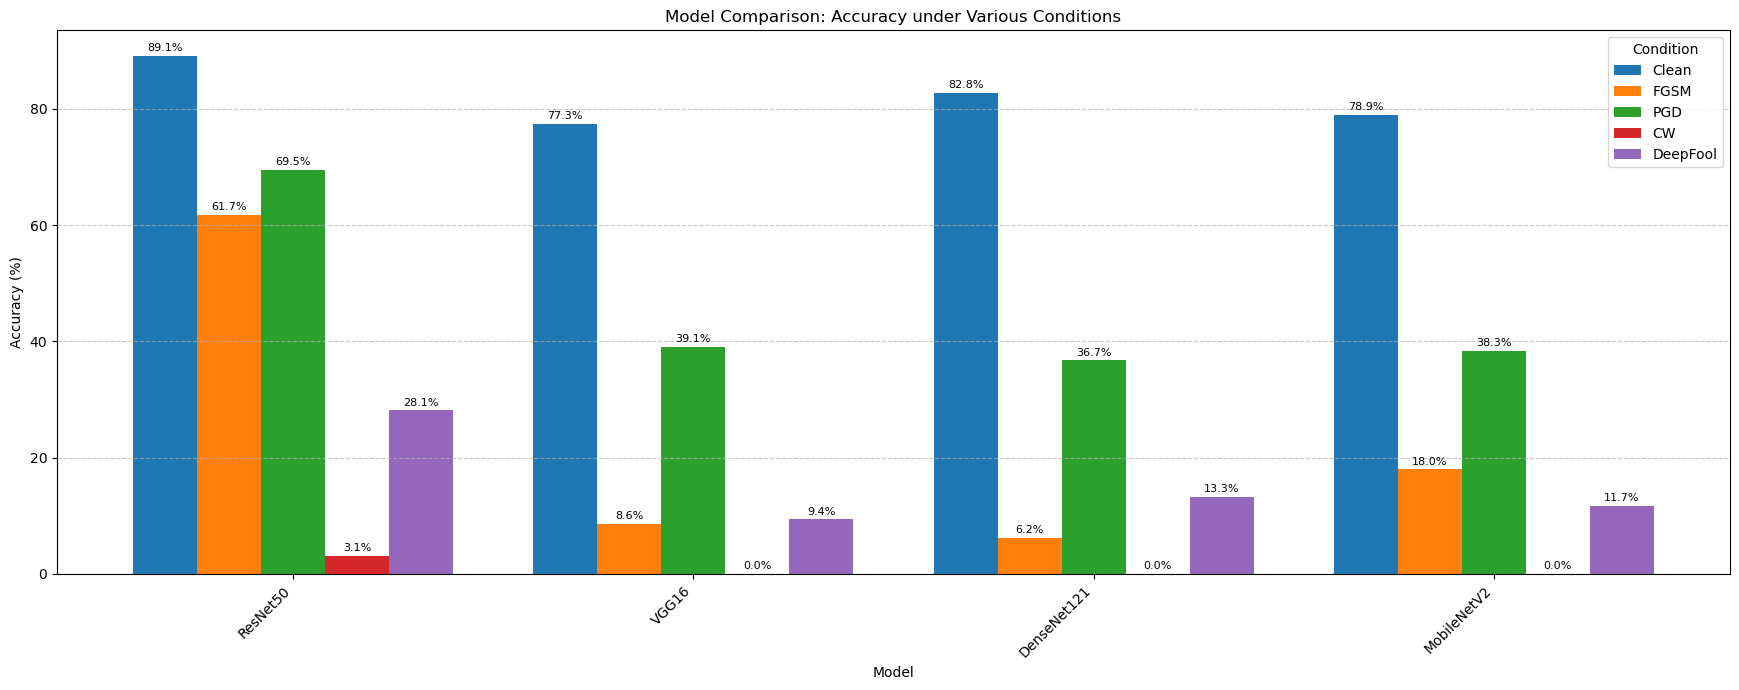
\includegraphics[width=1\textwidth]{model_comparison.png} % Przykładowy wykres
    \caption{Wpływ różnych ataków na dokładność klasyfikacji (przy $\epsilon = 0.03$)}
\end{figure}

\begin{table}[H]
    \centering
    \begin{tabular}{|l|c|c|c|c|c|}
    \hline
    \textbf{Model} & \textbf{Clean} & \textbf{FGSM} & \textbf{PGD} & \textbf{C\&W} & \textbf{DeepFool} \\
    \hline
    ResNet50 & 89.1\% & 61.7\% & 69.5\% & 3.1\% & 28.1\% \\
    VGG16 & 77.3\% & 8.6\% & 39.1\% & 0\% & 9.4\% \\
    DenseNet121 & 82.8\% & 6.2\% & 36.7\% & 0\% & 13.3\% \\
    MobileNetV2 & 78.9\% & 18.0\% & 38.3\% & 0\% & 11.7\% \\
    \hline
    \end{tabular}
    \caption{Spadek dokładności modeli po ataku}
\end{table}

Można przede wszystkim zauważyć wyraźny spadek po przeprowadzeniu ataków. Na pierwszy rzut oka widać pewnego rodzaju tendencje — ResNet50 zdecydowanie najlepiej poradził sobie z atakiem. Z drugiej strony, każda sieć praktycznie poległa po zastosowaniu ataku C\&W.

\begin{figure} [H]
    \centering
    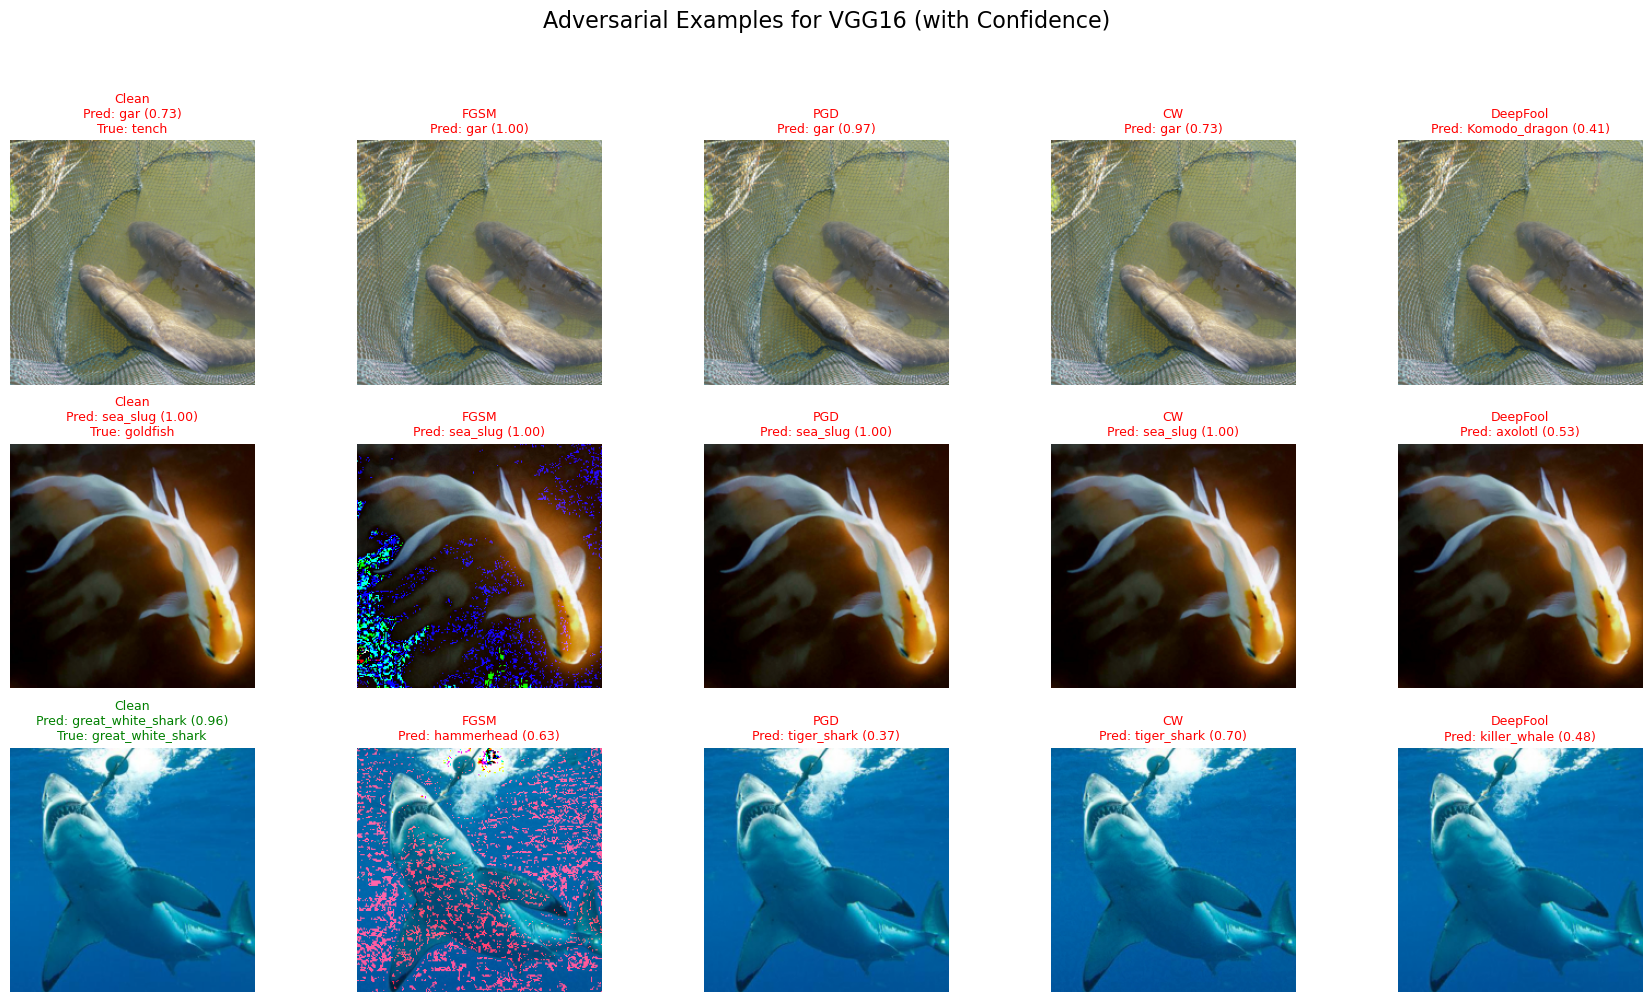
\includegraphics[width=1\textwidth]{adversarial_examples.png}
    \caption{Wizualna różnica pomiędzy obrazkami - przed i po atakach}
    \label{fig:enter-label}
\end{figure}

Widok obrazków porównawczych jednak rzuca też inną perspektywę — ludzką. Jak widać, FGSM zmienia wygląd obrazu dla ludzkiego oka. Przy innych atakach zmiany są praktycznie niewidoczne — gołym okiem nie jesteśmy w stanie stwierdzić, czy obrazek faktycznie został zaatakowany.
\subsection{Ataki hiperspektralne}

Ataki hiperspektralne w kontekście sieci konwolucyjnych (CNN) odnoszą się do manipulacji obrazów hiperspektralnych w celu oszukania modeli uczenia maszynowego, które je analizują. Obrazy hiperspektralne zawierają setki pasm spektralnych dla każdego piksela, co daje bardzo szczegółowe informacje o materiale czy strukturze obiektu. CNN, używane do klasyfikacji takich obrazów, mogą być podatne na ataki polegające na subtelnych zmianach w wybranych pasmach, które są niewidoczne dla człowieka, ale prowadzą model do błędnych decyzji. Tego typu ataki wykorzystywane są do testowania odporności systemów rozpoznawania obrazów w zastosowaniach takich jak monitoring środowiska, rozpoznanie wojskowe czy inspekcja przemysłowa.

\begin{figure}[H]
    \centering
    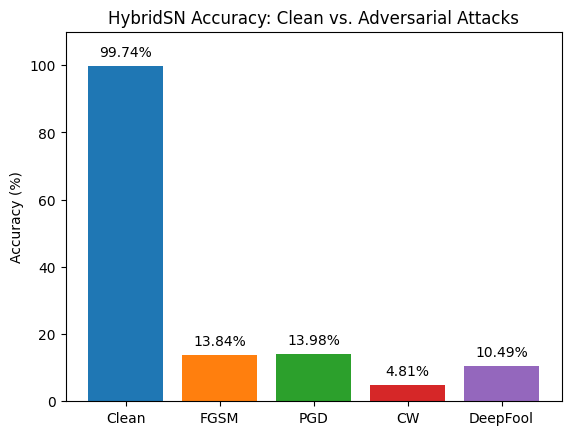
\includegraphics[width=1\textwidth]{hybridsn_accuracy.png} 
    \caption{Porównanie dokładności różnych ataków hiperspektralnych}
\end{figure}

Można zauważyć, że C\&W znowu dał najlepszy wynik (mniejsza dokładność — lepsza skuteczność ataku). Pozostałe ataki dały dość podobny poziom, jednak dalej na tyle wysoki, żeby faktycznie dać niepoprawny odczyt przy próbie klasyfikacji obrazów.

\begin{figure}[H]
    \centering
    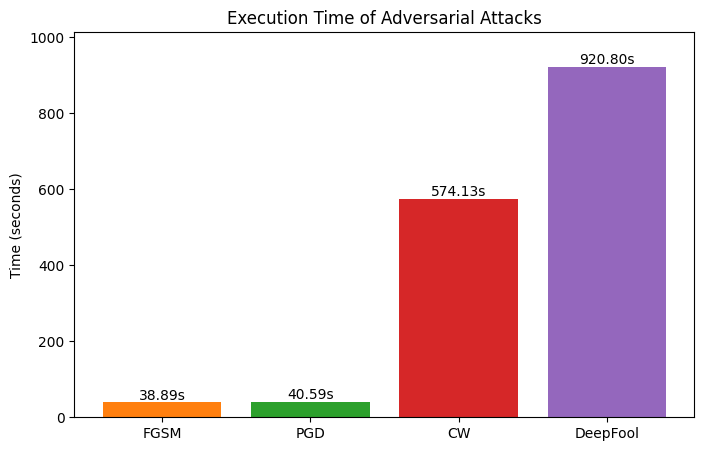
\includegraphics[width=1\textwidth]{hybridsn_time.png} 
    \caption{Porównanie czasu potrzebnego na dokonanie ataku hiperspektralnego}
\end{figure}

Jeśli chodzi o czas potrzebny na wykonanie ataków, widać podział na dwie grupy. FGSM oraz PGD wykonują się stosunkowo szybko — uzyskano czas poniżej minuty. Z kolei C\&W oraz DeepFool potrzebowały odpowiednio około 10 i 15 minut.

\begin{figure}[H]
    \centering
    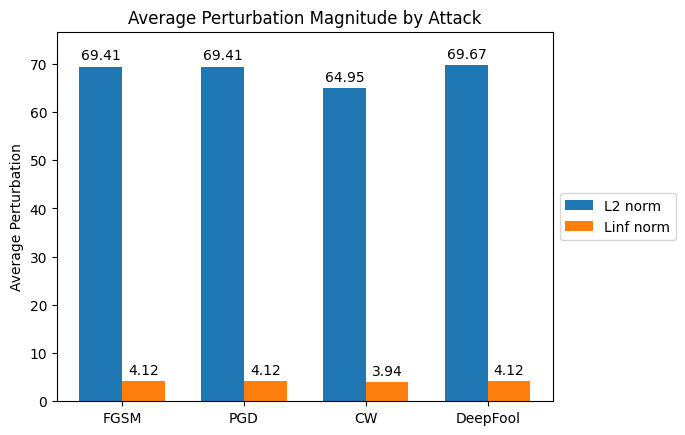
\includegraphics[width=1\textwidth]{perturbations.png} 
    \caption{Porównanie uzyskanych zaburzeń dla norm L2 i L$\infty$}
\end{figure}

Użyto dwóch norm:
\begin{itemize}
    \item norma L2 - mierzy całkowitą energię zaburzenia, czyli jego długość w przestrzeni euklidesowej. W praktyce oznacza to, że jeśli zaburzenie jest rozproszone równomiernie po wielu pikselach i pasmach spektralnych, ale o małej sile, to norma L2 będzie niska. Jest to często stosowane do oceny subtelnych, „gładkich” perturbacji.
    \item norma L$\infty$ - mierzy maksymalną zmianę wartości w jednym pikselu. Określa więc, jak bardzo zaburzenie może zmienić dowolną pojedynczą wartość w obrazie. Tę normę stosuje się, gdy celem jest ograniczenie „najgorszego przypadku” zmiany, nawet jeśli cała reszta obrazu pozostaje praktycznie nietknięta.
\end{itemize}
Wartości uzyskane są bardzo podobne, norma L2 dla C\&W jest trochę mniejsza, co może sugerować, że potrzebna była mniejsza czułość do skutecznego przeprowadzenia ataku. Uzyskane wyniki raczej pokazują odporność samego zbioru danych na ataki, niż skuteczność ich samą w sobie. Ogólnie więc możemy ten wykres interpretować tak, że potrzebne było dość duże zaburzenie globalne (norma L2) oraz że zmiana lokalna (maksymalna dla pojedynczego piksela) może być widoczna, jednak raczej dla obrazów o niższej rozdzielczości (L$\infty$).

\subsection{Kompresja JPEG a wpływ na wynik ataków adversarialnych}

\begin{figure} [H]
    \centering
    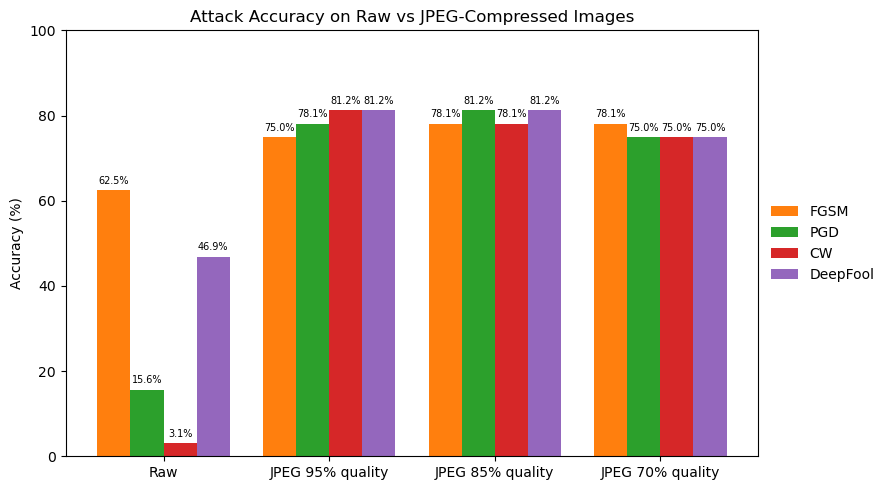
\includegraphics[width=1\textwidth]{jpeg_accuracy.png}
    \caption{Porównanie wyników po skompresowaniu zaatakowanych grafik w sieci ResNet50}
    \label{fig:enter-label}
\end{figure}

Po kompresji JPEG dla zaatakowanych obrazów, możemy zauważyć ciekawe wnioski — otóż działanie to dość silnie potrafi ograniczyć efekt samego ataku. Po konwersji stratnej uzyskano dokładność na poziomie około 80\%, co dla C\&W oznacza wzrost o 78 punktów procentowych. Dlaczego tak się dzieje? Głównie z dwóch powodów:
\begin{itemize}
    \item JPEG usuwa wysokoczęstotliwościowe szczegóły z obrazu — co dla przykładu metody ataków takie jak FGSM czy PGD robią.
    \item Kompresja ,,wygładza'' obraz — przy obrazach o niższej rozdzielczości nałożone perturbacje mogą się rozmyć.
\end{itemize}
Jednak dalej należy pamiętać, że JPEG jest konwersją stratną — nie wszystkie obrazy mogą zostać zapisane w tym formacie. Warto też pamiętać, że same ataki można dostosować pod ten format, co zniwelowałoby efekt końcowy.

\section{Analiza wyników}

Z przedstawionych wyników wynika, że skuteczność ataków adversarialnych znacząco różni się w zależności od użytego modelu i rodzaju ataku. Najważniejsze obserwacje to:

\begin{itemize}
    \item \textbf{ResNet50} wykazuje największą odporność na większość ataków. Dla ataku PGD dokładność spadła do 69{,}5\%, co nadal jest relatywnie wysokim wynikiem w porównaniu do innych modeli. Również przy ataku FGSM ResNet50 zachowuje stosunkowo dobrą skuteczność (61{,}7\%).
    
    \item \textbf{Atak Carlini \& Wagner (C\&W)} okazał się najskuteczniejszy – doprowadził do niemal całkowitej dezintegracji wszystkich modeli (dokładność od 0\% do 3{,}1\%). Świadczy to o jego precyzyjnej konstrukcji i zdolności do tworzenia zaburzeń minimalnie wpływających na percepcję wizualną, ale bardzo skutecznych wobec klasyfikatorów.
    
    \item \textbf{Modele VGG16, DenseNet121 oraz MobileNetV2} cechuje znacznie niższa odporność na ataki w porównaniu do ResNet50. VGG16, na przykład, osiąga zaledwie 8{,}6\% dokładności przy ataku FGSM i całkowicie zawodzi przy ataku C\&W.
    
    \item \textbf{DeepFool} osiąga umiarkowaną skuteczność — dokładność po ataku waha się od 9{,}4\% do 28{,}1\%. Ciekawym spostrzeżeniem jest jego wizualna subtelność, mimo że potrafi znacząco zaburzyć klasyfikację.
    
    \item \textbf{Hiperspektralne ataki} wykazały podobne właściwości — ataki C\&W ponownie były najskuteczniejsze, co potwierdza ich uniwersalność. Natomiast czas ich wykonania oraz poziom wymaganych zaburzeń wskazują na kompromis pomiędzy skutecznością a kosztami obliczeniowymi.
    
    \item \textbf{Kompresja JPEG} okazuje się być interesującą metodą obrony — znacząco redukuje wpływ ataku, szczególnie dla C\&W, gdzie dokładność wzrosła z 3{,}1\% do około 80\%. Oznacza to, że nawet proste techniki przetwarzania obrazu mogą w pewnych przypadkach niwelować efekty perturbacji.
\end{itemize}

\section{Wnioski}

Przeprowadzone eksperymenty pozwalają sformułować kilka kluczowych wniosków:

\begin{itemize}
    \item \textbf{Każdy model CNN jest podatny na ataki adversarialne}, jednak odporność na nie różni się znacznie w zależności od architektury. ResNet50 okazał się być najbardziej odporny, co może wynikać z jego głębokiej struktury rezydualnej, wspierającej lepsze generalizowanie.

    \item \textbf{Ataki optymalizacyjne}, takie jak Carlini \& Wagner, są najbardziej skuteczne, ale także najbardziej czasochłonne. Z kolei ataki jednokrokowe, jak FGSM, są szybkie, lecz często mniej efektywne — szczególnie wobec lepiej uodpornionych modeli.

    \item \textbf{Nawet niewidoczne dla ludzkiego oka perturbacje mogą prowadzić do drastycznych błędów klasyfikacji}, co potwierdzają wyniki DeepFool i C\&W. Wizualna niepozorność ataków stanowi istotne zagrożenie w zastosowaniach krytycznych, takich jak medycyna czy bezpieczeństwo.

    \item \textbf{Kompresja stratna JPEG może służyć jako prosta technika obronna}, ograniczając skuteczność ataków poprzez usunięcie zakodowanych w wysokich częstotliwościach perturbacji. Jest to obiecujący kierunek do dalszych badań nad preprocessingiem defensywnym.

    \item \textbf{W kontekście obrazów hiperspektralnych} — mimo większej liczby kanałów, modele CNN są nadal podatne na ataki, co wymaga opracowania specjalizowanych metod zabezpieczających, szczególnie w dziedzinach o wysokim znaczeniu (monitoring, obrona, przemysł).
\end{itemize}

Ostatecznie, skuteczna ochrona przed atakami adversarialnymi wymaga podejścia wielowarstwowego: od projektowania odpornych architektur, przez regularizację treningu, po zastosowanie prostych metod przetwarzania, takich jak kompresja JPEG.

\printbibliography

\end{document}